\documentclass{rescience}
\usepackage{array,booktabs,graphicx}
\setlength{\emergencystretch}{2em}
\rhead{} % A staged draft has not been submitted or placed under review.
\begin{document}
%% ----------------------------------------------------------------------------
%% ReScience article template
%% Copyright (c) 2018 N.P. Rougier,
%% Released under a Creative Commons Attribution 4.0 International license.
%% ----------------------------------------------------------------------------

%% --- Top left header --------------------------------------------------------
\begin{tikzpicture}[remember picture, overlay]
  \node [shape=rectangle, draw=darkred, fill=darkred, yshift=-34mm,
        anchor=north west, minimum width=3.75cm, minimum height=10mm]
        at (current page.north west) {};
  \node [text=white, anchor=center, yshift=-39mm, xshift=1.875cm]
         at (current page.north west) {\small \SpaceRoboto RESCIENCE C};
\end{tikzpicture}


%% --- Title -------------------------------------------------------------------
{\let\newpage\relax\maketitle} \maketitle


%% --- Margin information -----------------------------------------------------
\marginnote{
  \footnotesize \sffamily
  \ifdefempty{\editorNAME}{}{\textbf{Edited by}\\
  \editorNAME\ifdefempty{\editorORCID}{}{$^{\orcid{\editorORCID}}$}\\
  ~\\}
  %%
  \ifdefempty{\reviewerINAME}{}
  {
  \textbf{Reviewed by}\\
  \ifdefempty{\reviewerINAME}{\textcolor{darkgray}{}}
             {\reviewerINAME\ifdefempty{\reviewerIORCID}{}{$^{\orcid{\reviewerIORCID}}$}\\}
  \ifdefempty{\reviewerIINAME}{\textcolor{darkgray}{}}
             {\reviewerIINAME\ifdefempty{\reviewerIIORCID}{}{$^{\orcid{\reviewerIIORCID}}$}\\}
  ~\\
  }
  %%           
  \textbf{Received}\\
  \ifdefempty{\dateRECEIVED}{---}{\dateRECEIVED}\\
  ~\\
  %%
  \textbf{Published}\\
  \ifdefempty{\datePUBLISHED}{---}{\datePUBLISHED}\\
  ~\\
  %%
  \textbf{DOI}\\
  \ifdefempty{\articleDOI}{---}{\articleDOI}
}
 

%% --- Bottom statement -------------------------------------------------------
\newcommand{\container}[1]{\def\@container{#1}}
\begin{container}
  \afterpage {
    \begin{statement}
      \scriptsize \sffamily
      \hrule \vskip .5em
      Copyright © \articleYEAR~\authorsABBRV,
      released under a Creative Commons Attribution 4.0 International license.
      
      Correspondence should be addressed to
      \contactNAME~(\href{mailto:\contactEMAIL}{\contactEMAIL})
  
      % Competing-interest declaration requires author confirmation; no default assertion inserted.

      \ifdefempty{\codeURL}{}
      {Code is available at
      \href{\codeURL}{\detokenize\expandafter{\codeURL}}\ifdefempty{\codeDOI}{.}{ -- DOI \doi{\codeDOI}.}\ifdefempty{\codeSWH}{.}{ -- SWH  \href{https://archive.softwareheritage.org/\codeSWH/}{\detokenize\expandafter{\codeSWH}}.}}

      \ifdefempty{\dataURL}{}
      {Data is available at
      \href{\dataURL}{\detokenize\expandafter{\dataURL}}\ifdefempty{\dataDOI}{.}{ -- DOI \doi{\dataDOI}.}}

      \ifdefempty{\reviewURL}{}
     {Open peer review is available at \href{\reviewURL}{\detokenize\expandafter{\reviewURL}}.}
    \end{statement}
  }
\end{container}


%% --- Abstract ---------------------------------------------------------------
%% \ifdefempty{\articleABSTRACT}{}{
%%   {\small \sffamily \textbf{Abstract} \articleABSTRACT \par}
%% }


%% --- Replication ------------------------------------------------------------
%% \ifdefempty{\replicationBIB}{}{
%%   {\small \sffamily \bfseries A replication of}
%%   \ifdefempty{\replicationURL}
%%        {\href{http://doi.org/\replicationDOI}{\small \sffamily \replicationBIB}}
%%        {\href{\replicationURL}{\small \sffamily \replicationBIB}}.
%% \par }

\section*{Abstract}
Learning-augmented priority queues can reduce expensive true-key comparisons, but replicating that result requires precise advice, tie and counting conventions. We partially replicate the sorting experiments of Benomar and Coester with an independently authored C++ implementation checked against their released Python code. Across 11,340 runs, the class-quality and decay responses agree with the original findings; median pointwise relative errors are below 0.16\% on every curve at the two main-paper sizes. Comparison benefits remain conditional on advice quality, with the uninformative class endpoint exceeding the analytic heap reference. A separate extension identifies historical node-map ownership: last-occurrence cleanup reduces drained-queue traced memory from 35.18 to 0.024 MiB, with the ownership effect repeated on a second host. Native graph controls favor a direct heap on all seven tested workloads on both hosts. The artifact separates replicated comparison-count evidence from these additional memory and runtime measurements and provides reproducible input generation, raw counts and verification procedures.
\section{Scope and original result}
Benomar and Coester study priority queues augmented by pointer predictions, rank predictions, and dirty comparisons \cite{ref1}. Their sorting experiments measure clean key comparisons, rather than elapsed time. We target the three learning-augmented curves in Figures 2 and 3 of Section 5 and Figures 6 and 7 of Appendix F.1. This is a partial replication: the Fibonacci-heap and Bai–Coester sorting implementations, the graph experiments, and the theoretical proofs are outside the replicated subset.

The comparison-count model is valuable when true comparisons are costly. Predictions and integer-index operations have a different cost in that model. The replication therefore preserves the original metric; it does not reinterpret a reduction in clean comparisons as a claim of faster wall-clock execution. After the replication, Section 5 examines historical node-map retention and its repair in the same artifact; Section 6 reports native runtime controls on two physical hosts.

We reconstruct the methods from the paper and consult the released implementation to resolve details of ties, prediction generation, sentinel comparisons, and search behavior \cite{ref1,ref2}. The new engine is separately authored C++; it is not a clean-room implementation. The artifact records these dependencies and provides a small differential correctness gate against the pinned Python source.

Algorithms with predictions combine useful advice with guarantees under error: caching is an early example \cite{ref10}, and Mitzenmacher and Vassilvitskii survey the broader framework \cite{ref11}. Empirical priority-queue studies emphasize that implementation and workload choices affect practical costs \cite{ref3,ref6}. Learned-index benchmarks evaluate prediction machinery against conventional indexes \cite{ref7}; later studies examine when learned indexes help and compare learned, compressed and traditional integer indexes \cite{ref8,ref9}. These works motivate separating the replicated clean-comparison model from the memory/runtime extension. We reproduce a specific published sorting result, without proposing a new asymptotic queue bound or transferring learned-index benchmark conclusions directly to priority queues.

\section{Reconstruction and comparison accounting}
All sorting inputs contain distinct true keys. Offline predictions determine a stable order of insertion, with the previously inserted node used as the next search hint. Online rank predictions accompany keys in a uniformly random insertion order. The dirty/clean model first searches using predicted-order comparisons and then corrects that location using true comparisons. Tied advice and negative predicted ranks are retained.

We count true-key comparisons in skip-list search and correction, matching the released convention that comparisons with the head sentinel are free. Dirty comparisons are recorded separately. Sorting advice, querying the prediction-rank index, pointer manipulation, and validating the output are outside the clean-comparison count. Node heights follow the geometric distribution with promotion probability one half. Validation checks ordering and the exact comparator behavior on shared small inputs and heights.

The binary-heap curve is the authors' analytic reference, calculated from their released expression \cite{ref2}. It is not a measured binary-heap implementation. We report ratios to that reference and the parameter intervals where they cross one, without assuming that every prediction quality beats it.

\section{Experimental protocol and published reference}
The grid uses n = 1,000, 10,000 and 100,000 distinct keys and 21 parameter values per prediction setting. Let T be floor(n sqrt(n)). At grid index i from 0 to 20, the class parameter is floor(i n / 20) and the decay parameter is floor(i T / 20). Each algorithm and cell receives 30 independent replicates. The n = 1,000 curves provide the released aggregate anchor, while the larger sizes target the main paper's figures. Seeds, generated-input hashes, code hashes and completeness checks accompany the observations.

The artifact clamps the plotted class parameter zero to one class. Its random cutpoints can coincide with the zero endpoint, so even the largest plotted class parameter is not defined as perfectly accurate advice. Decay starts from true ranks and perturbs uniformly selected items by a fair signed unit step. We preserve these conventions rather than silently substituting a different prediction generator.

For efficient endpoint generation, the decay implementation samples the counts of the 2n signed item categories from a multinomial distribution, then applies each item's positive minus negative count to its true rank. This has the same mathematical endpoint law as literal independent perturbation steps because sorting observes only the final ranks. The floating-point sampler and random-number stream differ from the released generator; no bitwise same-seed agreement is claimed. A literal mode supports small validation cases.

The pinned repository contains mean and standard-deviation arrays for the three learned methods at n = 1,000, but no corresponding per-run observations. Published curves at the larger sizes are recovered from the final PDF's vector paths using calibrated axis ticks. The original paper states that each plotted point averages 30 independent runs; the effective number of runs underlying the released aggregate files cannot be verified from those files. Aggregate dispersion is not treated as a known standard error. We report pointwise relative differences and descriptive whole-curve errors, retaining all parameter values and identifying uncertainty from the new replicates separately.

The assessment is claim-specific: class-quality response, decay response, ratios to the analytic heap reference, and differences among prediction models. No arbitrary numerical agreement threshold determines a single success score. A failure to match one curve is investigated against generator, comparator and extraction conventions before it is interpreted as a failure to replicate the published finding.

The primary engine is separately authored C++17. Before execution, 666 small shared-input cases matched the pinned Python sorting functions exactly in cumulative clean and dirty counts and in complete comparator-call trace digests. The optimized and AddressSanitizer/UndefinedBehaviorSanitizer builds both passed. Four malformed-input controls failed closed, and six checks matched the released analytic heap expression.

Within each new condition, the three methods share the final rank-advice array, the geometric-height sequence by insertion step, and the insertion permutation where applicable. Offline sorting instead stably orders the ordinal keys by advice. Repetitions and parameter cells use independent, domain-separated advice, order and height streams. This pairing preserves each method's marginal experiment while differing from the original unseeded, interleaved algorithm loops.

The condition grid, source hashes, claim-specific analysis rules and published references were privately frozen before primary execution. This is a documented computational freeze, not an externally registered preregistration. The run executed on the Apple M1 MacBook Air under CPython 3.13.3 and NumPy 2.2.4, using Apple Clang 15 with C++17, -O3 and -DNDEBUG. Each model record constructs fresh queue state and checks the entire ordinal output. No sorting wall-time claim is made.

Pointwise intervals use 5,000 deterministic percentile-bootstrap resamples of our thirty runs. Paired model ratios resample shared conditions together; endpoint contrasts resample independently seeded endpoint cells separately. Intervals are pointwise, without simultaneous coverage correction. Every planned cell and recorded failure is retained, and no parameter or seed was retuned after observing the primary counts.

\section{Replication results}
All 3,780 planned shared-input conditions and 11,340 model runs completed, with exact ordinal-output checks passing for every run. This yields 378 model/parameter means with 30 replicates each. The new records and all earlier graph timing records are kept separate.

The curves closely follow the published comparison-count behavior. Across the twelve curves at the two main-paper sizes, median pointwise absolute relative errors range from 0.028\% to 0.151\%; the largest individual relative error is 0.743\%. For the six 1,000-key released-aggregate curves, the largest individual error is 4.650\%. Table 1 reports every curve, including the smaller-size deviations.

\begin{table}[!htbp]\centering\footnotesize\setlength{\tabcolsep}{3pt}
\caption{Agreement of replicated means with the available references. At n = 1,000, reference values are released aggregate means; at larger sizes they are vector-derived plotted means from the final paper. Relative errors use the reference mean as denominator. Normalized RMSE is whole-curve RMSE divided by the arithmetic mean of its 21 reference means. These are descriptive agreement measures.}
\begin{tabular}{@{}>{\raggedright\arraybackslash}p{\dimexpr 0.14798206278026907\linewidth-2\tabcolsep\relax}>{\raggedright\arraybackslash}p{\dimexpr 0.11883408071748879\linewidth-2\tabcolsep\relax}>{\raggedright\arraybackslash}p{\dimexpr 0.15022421524663676\linewidth-2\tabcolsep\relax}>{\raggedright\arraybackslash}p{\dimexpr 0.1905829596412556\linewidth-2\tabcolsep\relax}>{\raggedright\arraybackslash}p{\dimexpr 0.1905829596412556\linewidth-2\tabcolsep\relax}>{\raggedright\arraybackslash}p{\dimexpr 0.20179372197309417\linewidth-2\tabcolsep\relax}@{}}\toprule
Setting & n & Model & Median rel. error (\%) & Max rel. error (\%) & Normalized RMSE (\%) \\\midrule
Class & 1,000 & Offline & 0.590 & 4.650 & 2.986 \\
Class & 1,000 & Online & 0.813 & 3.517 & 1.773 \\
Class & 1,000 & Dirty/clean & 0.681 & 2.030 & 1.116 \\
Class & 10,000 & Offline & 0.151 & 0.743 & 0.700 \\
Class & 10,000 & Online & 0.113 & 0.621 & 0.503 \\
Class & 10,000 & Dirty/clean & 0.101 & 0.596 & 0.738 \\
Class & 100,000 & Offline & 0.059 & 0.307 & 0.605 \\
Class & 100,000 & Online & 0.064 & 0.309 & 0.449 \\
Class & 100,000 & Dirty/clean & 0.028 & 0.207 & 0.296 \\
Decay & 1,000 & Offline & 0.646 & 2.189 & 1.004 \\
Decay & 1,000 & Online & 0.609 & 2.122 & 1.015 \\
Decay & 1,000 & Dirty/clean & 0.335 & 2.806 & 1.046 \\
Decay & 10,000 & Offline & 0.094 & 0.335 & 0.164 \\
Decay & 10,000 & Online & 0.067 & 0.450 & 0.195 \\
Decay & 10,000 & Dirty/clean & 0.087 & 0.259 & 0.135 \\
Decay & 100,000 & Offline & 0.032 & 0.124 & 0.055 \\
Decay & 100,000 & Online & 0.039 & 0.089 & 0.049 \\
Decay & 100,000 & Dirty/clean & 0.033 & 0.092 & 0.048 \\
\bottomrule\end{tabular}\end{table}
Figures 1 and 2 overlay the independently generated means and the published references at the main-paper sizes. Solid lines with open markers show this replication; dashed lines show the published means. The narrow shaded bands are pointwise 95\% bootstrap intervals from our 30 replicates. No original standard errors or distributional-equivalence claim are inferred from these overlays.

\begin{figure}[!htbp]\centering
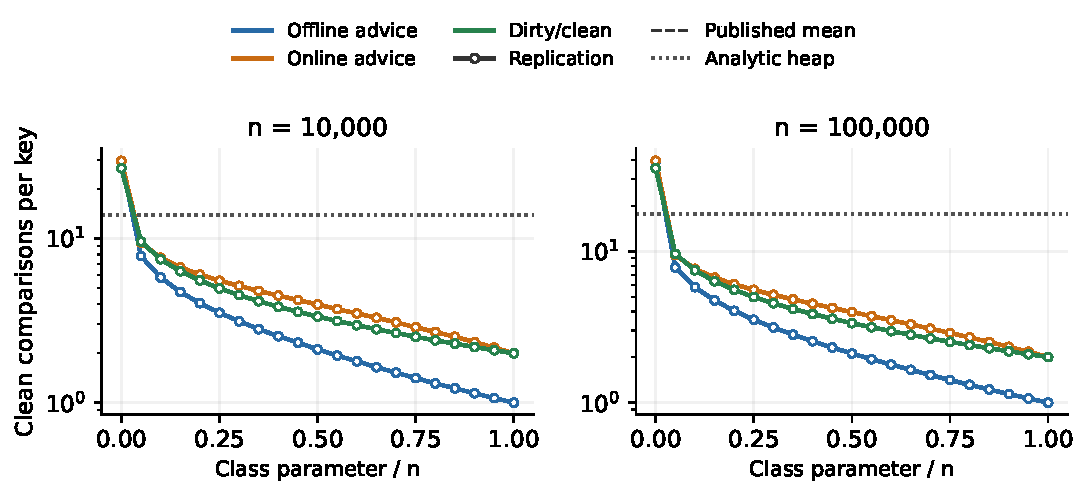
\includegraphics[width=\linewidth]{figure-9bb7cec14f6a.pdf}
\caption{Partial replication of the original Figure 2: clean comparisons per key under class predictions. Both ordinate axes are logarithmic. The plotted class parameter zero is implemented as one class. Published and replicated curves largely overlap at this scale. The dotted horizontal line is the released analytic binary-heap reference, not a timed heap.}
\end{figure}
\begin{figure}[!htbp]\centering
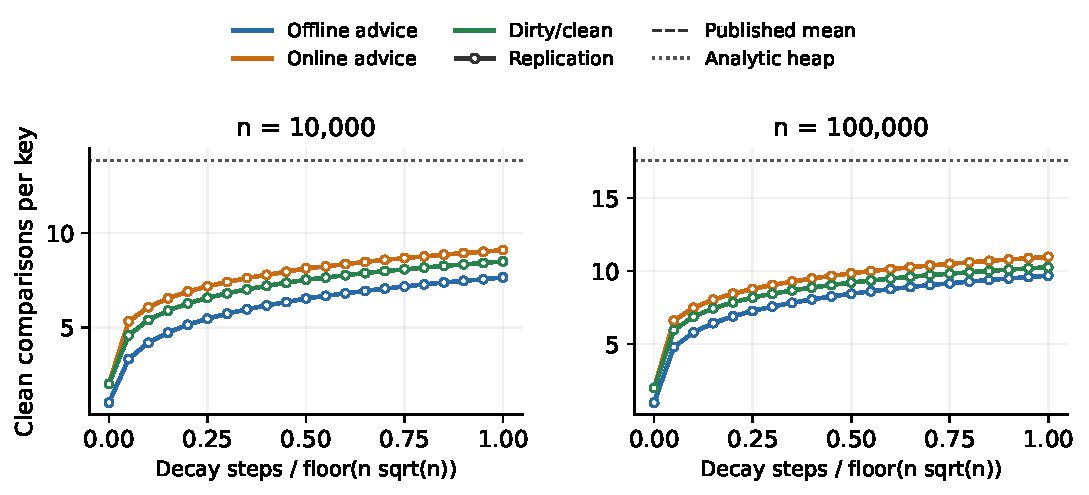
\includegraphics[width=\linewidth]{figure-12c3be78ca02.pdf}
\caption{Partial replication of the original Figure 3: clean comparisons per key under decay predictions. The horizontal coordinate divides the timestep parameter by floor(n sqrt(n)); this rescales the original main-paper axis without changing the experiments. Better advice is at the left. Published and replicated curves largely overlap at this scale. The dotted line is the analytic binary-heap reference.}
\end{figure}
All eighteen endpoint contrasts have the expected direction: increasing the class parameter from its first to last value reduces the mean clean count, while increasing decay from zero to its maximum increases it, for all three methods and all three sizes. Each pointwise 95\% bootstrap interval for the endpoint difference excludes zero in that direction.

\begin{table}[!htbp]\centering\footnotesize\setlength{\tabcolsep}{3pt}
\caption{Replicated mean clean comparisons per key at the first and last parameter values. Class start/end correspond to plotted c = 0/n; decay start/end correspond to t = 0/floor(n sqrt(n)). The full pointwise and endpoint interval tables are in the artifact.}
\begin{tabular}{@{}>{\raggedright\arraybackslash}p{\dimexpr 0.10089686098654709\linewidth-2\tabcolsep\relax}>{\raggedright\arraybackslash}p{\dimexpr 0.14573991031390135\linewidth-2\tabcolsep\relax}>{\raggedright\arraybackslash}p{\dimexpr 0.14798206278026907\linewidth-2\tabcolsep\relax}>{\raggedright\arraybackslash}p{\dimexpr 0.14798206278026907\linewidth-2\tabcolsep\relax}>{\raggedright\arraybackslash}p{\dimexpr 0.14798206278026907\linewidth-2\tabcolsep\relax}>{\raggedright\arraybackslash}p{\dimexpr 0.14798206278026907\linewidth-2\tabcolsep\relax}>{\raggedright\arraybackslash}p{\dimexpr 0.16143497757847533\linewidth-2\tabcolsep\relax}@{}}\toprule
n & Model & Class start & Class end & Decay start & Decay end & Analytic BH \\\midrule
1,000 & Offline & 19.740 & 1.000 & 0.999 & 5.736 & 9.954 \\
1,000 & Online & 19.948 & 1.989 & 1.985 & 7.321 & 9.954 \\
1,000 & Dirty/clean & 18.516 & 1.987 & 1.985 & 6.731 & 9.954 \\
10,000 & Offline & 29.698 & 1.000 & 1.000 & 7.647 & 13.854 \\
10,000 & Online & 29.738 & 1.998 & 1.998 & 9.099 & 13.854 \\
10,000 & Dirty/clean & 26.801 & 1.998 & 1.998 & 8.498 & 13.854 \\
100,000 & Offline & 39.497 & 1.000 & 1.000 & 9.681 & 17.557 \\
100,000 & Online & 39.573 & 2.000 & 2.000 & 10.968 & 17.557 \\
100,000 & Dirty/clean & 35.305 & 2.000 & 2.000 & 10.262 & 17.557 \\
\bottomrule\end{tabular}\end{table}
The advantage over the analytic heap reference depends on advice quality. Pointwise bootstrap intervals lie below that reference in 369 of 378 cells. The nine remaining cells are the lowest-quality class endpoint, across all three sizes and methods; their intervals lie above it. All twenty other sampled class levels and all sampled decay levels lie below the reference. Thus the replication supports substantial comparison-count benefits over the tested useful-advice range while preserving the unfavorable uninformative-class endpoint visible in the original curves.

The relative ordering of prediction interfaces is also preserved: at the highest class parameter and at zero decay, offline advice requires about one clean comparison per key, and online and dirty/clean advice require about two. Model-to-model paired ratios and every observed heap-crossing bracket are reported in the artifact. The original qualitative description of comparable performance is not converted into an arbitrary numerical equivalence margin.

Original per-run observations and random states are not provided in the pinned artifact. The paper states a nominal thirty runs per plotted point, while the saved 1,000-key aggregates do not document their effective trial count. The published n = 100,000 class heap line corresponds to approximately 17.557000 comparisons per key; the released analytic expression gives 17.557310. We retain that small plot/reference discrepancy and calibrate the vector-derived means using the printed axis ticks, rather than adjusting a scale to force agreement.

\section{Retention in the replicated artifact and its repair}
The comparison-count replication also makes the released implementation's object ownership relevant: extracting a key need not release the references held by the queue. We therefore examine a retention bug in the same pinned Python artifact \cite{ref2}. This is an additional implementation finding, not a failure of the replicated comparison-count result or its theoretical model.

Appendix C.1 describes collecting equal-priority items behind one ordered key \cite{ref1}. The released OnlineSL does not implement that grouping: it creates a skip-list node on each insertion, including repeated priorities \cite{ref2}. Its rank/value occurrence lists and Dijkstra routing buckets do not suppress those insertions. The repair below retains this one-node-per-insertion policy; grouped implementations are separate controls.

Along a successful execution with finite numeric priorities, let H be the number of distinct priorities inserted during the lifetime of an original queue. The released implementation assigns each newly encountered priority an entry in sl.nodes and never erases that entry during deletion. Starting from an empty map, induction on insertions and extractions gives H map entries after the queue drains. Consequently, this metadata has an \(\Omega(H)\) entry-count lower bound even when the maximum number of simultaneously live queue entries is fixed. 

The fix deletes a priority's sl.nodes mapping only after its final live occurrence is extracted. Hint selection reads the map using a key from a nonempty live rank bucket; with consistent occurrence bookkeeping, an exhausted key cannot be selected by that path. Reinsertion installs a new mapping before the key can supply a later hint. The fix leaves node links intact. An extracted duplicate can still be the mapped representative of another live occurrence, so clearing its links is unsafe: insert 1 twice, extract once, then insert 2 with identity advice and height seed 101. The original and map-cleaned queues give 1, 1, 2; our rejected link-detachment variant raises IndexError. This counterexample concerns that modification, not the original queue. The upstream report supplies a reproducer and the ownership explanation \cite{ref12}.

A bounded-live experiment isolates ownership from graph size and duplicate grouping. It inserts unique increasing priorities with constant rank zero and an index universe of one, keeping at most 128 entries live. Each method/length/GC-mode case runs in a fresh process, with tracing started after imports and warmup. After draining the queue, we measure traced allocations while the empty queue remains alive, before and after explicit full garbage collection. Both hosts pass every expected-extraction check.

\begin{table}[!htbp]\centering\footnotesize\setlength{\tabcolsep}{3pt}
\caption{Drained-queue traced memory after 100,000 unique insertions with at most 128 live entries, after explicit full GC while the queue remains alive. Both columns use the same list rank buckets; only node-map ownership changes. Automatic GC enabled or disabled during the trace gives the same post-GC values on each host. These are retained allocations, not peak RSS, training memory or graph-query peaks.}
\begin{tabular}{@{}>{\raggedright\arraybackslash}p{\dimexpr 0.2790697674418604\linewidth-2\tabcolsep\relax}>{\raggedright\arraybackslash}p{\dimexpr 0.2325581395348837\linewidth-2\tabcolsep\relax}>{\raggedright\arraybackslash}p{\dimexpr 0.2325581395348837\linewidth-2\tabcolsep\relax}>{\raggedright\arraybackslash}p{\dimexpr 0.25581395348837205\linewidth-2\tabcolsep\relax}@{}}\toprule
Host & Retain history, MiB & Map cleanup, MiB & Node-map entries \\\midrule
Mac & 35.18 & 0.02386 & 100,000 to 0 \\
Windows + WSL2 & 34.42 & 0.02375 & 100,000 to 0 \\
\bottomrule\end{tabular}\end{table}
The large difference persists with automatic cyclic GC disabled; explicit full collections report zero collected objects. Thus the measured effect is historical ownership, not evidence of delayed cycle collection. The cleaned map is empty after draining, but the small remaining allocation includes queue/runtime state and is not a constant-space theorem. The supplement reports all lengths, GC snapshots and graph-memory cases, and separates map cleanup from bucket substitution and the coupled grouping/representative repair.

\section{Extensions: runtime on two hosts}
We separately measured compiled graph-query runtime on seven targets: Brussels, New York, a grid, a geometric graph, and three sparse-graph targets. Each has three training sources with one near and one far held-out query per source: 42 query/model cases, seven paired repetitions and 3,444 method timings per host. The radix heap is omitted for the twelve Brussels/geometric cases with floating weights; all other applicable methods receive seven repetitions. The first host is an Apple M1 MacBook Air with macOS 14.3.1 and Apple Clang 15; the second is an Intel Core i5-8365U Dell Latitude 5400 running Ubuntu 24.04 under Windows 11/WSL2 with g++ 13.3. Both use C++17, -O3 and -DNDEBUG without fast-math. All distances and drain checks pass against the same independent references.

The native controls are separately engineered grouped queues, not a timing rerun of the original Python classes. Plain and guided skip lists share live-key bookkeeping; guided variants use set/bitmap indexes and exact, linear or histogram advisors. A direct heap stores distance, reverse insertion sequence and vertex together, while a shared scalar heap uses the common distance-to-vertex routing map. These controls preserve LIFO ties and distinguish queue costs from routing-interface costs. Training and validation are outside query clocks; method order is randomized within host. Ratios are paired within repetition, repetitions collapse within each query/model case, and the six cases form each workload median.

\begin{table}[!htbp]\centering\footnotesize\setlength{\tabcolsep}{3pt}
\caption{Workloads on which the direct heap has the lowest native workload-level median among tested methods. These are descriptive counts for the seven fixed workloads, not independent-host confidence claims or universal rankings.}
\begin{tabular}{@{}>{\raggedright\arraybackslash}p{\dimexpr 0.42857142857142855\linewidth-2\tabcolsep\relax}>{\raggedright\arraybackslash}p{\dimexpr 0.2857142857142857\linewidth-2\tabcolsep\relax}>{\raggedright\arraybackslash}p{\dimexpr 0.2857142857142857\linewidth-2\tabcolsep\relax}@{}}\toprule
Host & CPU clock & Wall clock \\\midrule
Mac & 7 / 7 & 7 / 7 \\
Windows + WSL2 & 7 / 7 & 7 / 7 \\
\bottomrule\end{tabular}\end{table}
The direct-heap result persists on both hosts, while finer index and shared-heap comparisons can change direction. The supplement retains those exceptions, source-cluster intervals and all ablations; only three training clusters underlie each workload. Hosts are analyzed separately, since hardware, OS and compiler change together. Across the full extension, 12,300 graph-query timings are retained, separate from the 11,340 counted sorting records. Neither runtime results nor memory ownership replace the clean-comparison evidence replicated above.

\section{Limitations and conclusion}
The replication covers a specified sorting subset and a clean-comparison metric. It does not test every original algorithm, dataset or theorem. Published aggregate records and PDF coordinates offer less information than original per-run data. The independent implementation resolves documented ambiguities with the released source, and therefore shares those declared conventions. The separate practical-cost extension has a limited workload/host sample and does not establish universal runtime ordering.

Within the declared sorting subset, the comparison-count benefits replicate closely across both prediction-error models, three queue interfaces and three input sizes. The full curves preserve both useful-advice gains and the unfavorable uninformative-class endpoint. The independent implementation, explicit counting convention and published-reference extraction make that assessment reproducible. The separate ownership and native-runtime studies extend the artifact evaluation under different workloads and advice interfaces; they do not replace the original comparison metric or invalidate its theoretical cost model. For maintainers, the ownership fix is to delete a key's sl.nodes entry when its last live occurrence is extracted; node links can be left intact. The replication and extension together make both the published comparison result and practical implementation costs reproducible.

\section*{Artifact availability}
The accompanying artifact contains source, raw observations, input hashes, frozen computational plans, correctness checks, and reproduction commands. Upstream source and road data are fetched separately by pinned hashes. The feasibility pilot is excluded from reported counts. AI coding assistants were used as tools for code generation, debugging, and editing of prose. The author designed the experiments, ran all measurements on both hosts, verified all reported figures against the raw artifact, and is responsible for all claims.


\setlength\bibitemsep{0pt}
\printbibliography
\end{document}
